\subsubsection{Diagramma delle classi}

\begin{figure}[H]
    \centerfloat
    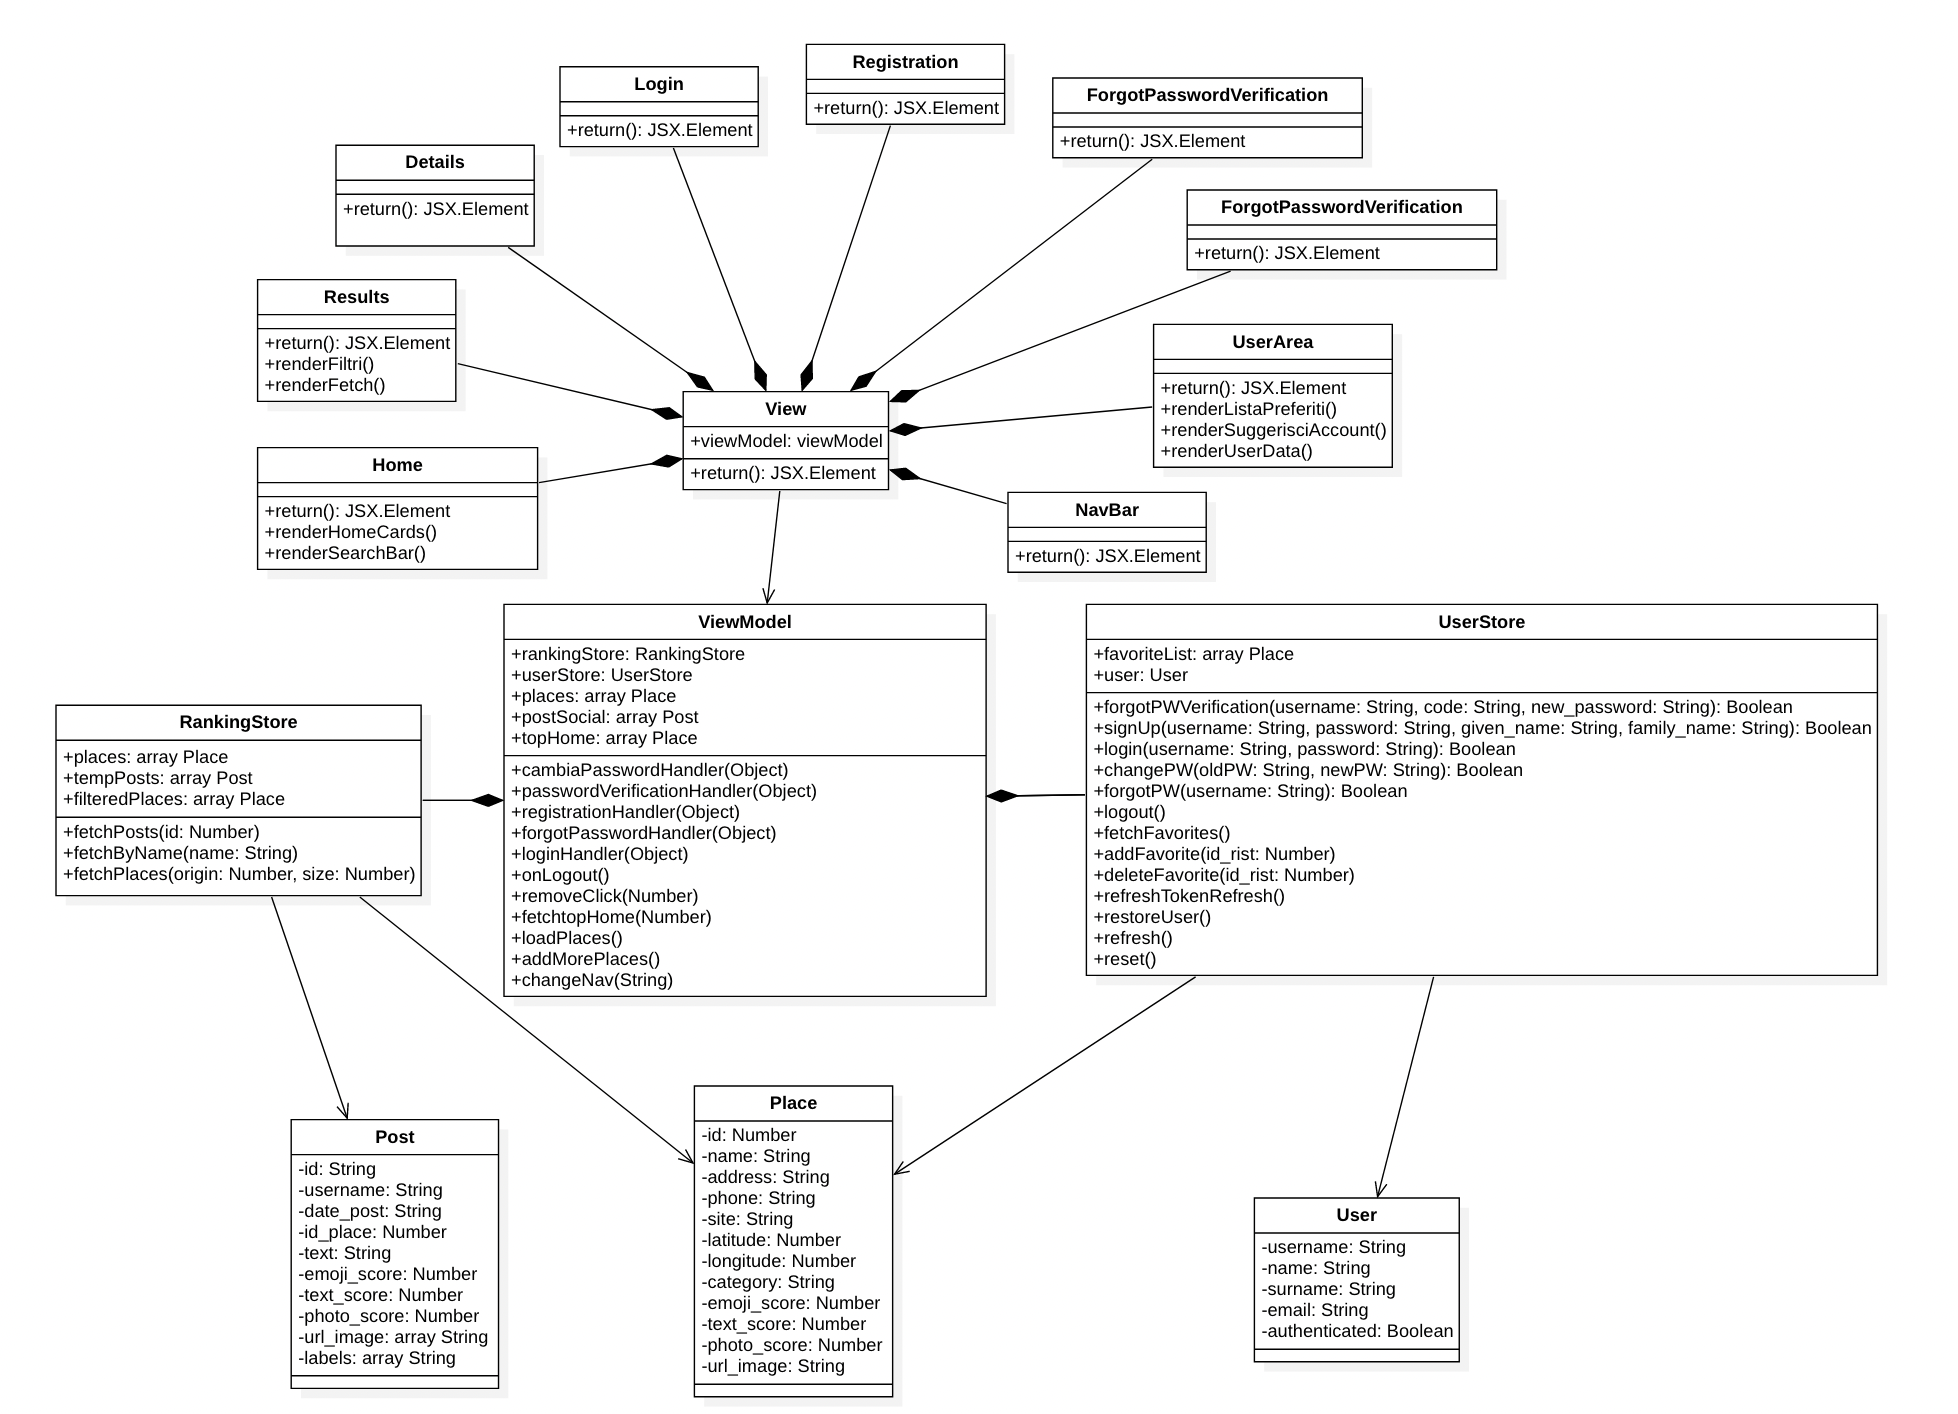
\includegraphics[scale=0.45]{Contenuto/Immagini/DiagrammaClassiFrontEnd.png}
    \caption{Architettura Frontend - Diagramma delle classi}
\end{figure}

\subsubsection{Diagramma di sequenza}

Abbiamo ritenuto non opportuno includere un diagramma di sequenza per la parte Frontend, perché le operazioni svolte risultano essere troppo semplici.

Infatti, le varie operazioni svolte lato Frontend sono delle semplici chiamate API (GET e POST) verso il Backend per ottenere i dati richiesti dall'utente (ad esempio i risultati che vengono mostrati dopo una ricerca oppure i migliori locali mostrati nella Home). Una volta ricevuto il responso dal Backend viene semplicemente aggiornata la vista della WebApp, come spiegato precedentemente.
